\documentclass{juliacon}

\setcounter{page}{1}

\begin{document}
% **************GENERATED FILE, DO NOT EDIT**************

\title{Kezdi.jl: A data analysis package for economists}

\author[1, 2, 3, 4]{Miklós Koren}
\author[1, 2]{Gergely Attila Kiss}
\affil[1]{Central European University, Vienna, Austria}
\affil[2]{HUN-REN KRTK, Budapest, Hungary}
\affil[3]{CEPR, London, United Kingdom}
\affil[4]{CESifo, Munich, Germany}

\keywords{Julia, Data analysis, Data wrangling, Stata}

\hypersetup{
pdftitle = {Kezdi.jl: A data analysis package for economists},
pdfsubject = {JuliaCon 2022 Proceedings},
pdfauthor = {Miklós Koren, Gergely Attila Kiss},
pdfkeywords = {Julia, Data analysis, Data wrangling, Stata},
}


\maketitle

\begin{abstract}
Economists overwhelmingly rely on proprietary data analysis languages such as Stata and MATLAB for their research computing needs. The transition to open-source languages like Julia presents various challenges due to differences in syntax, functionality, and best practices. We introduce \texttt{Kezdi.jl}, a data analysis package designed for economists that provides a Stata-like interface for working with data frames in Julia. The package is built on \texttt{DataFrames.jl} and related libraries, but uses a streamlined macro-based interface to eliminate common points of confusion. By emulating best practices from Stata, \texttt{Kezdi.jl} allows economists to be productive in Julia from day one. It supports a wide range of data wrangling and analysis tasks, including cleaning and transforming data, handling missing values, generating new variables, aggregating data, and running regressions.
\end{abstract}

\section{Introduction}

Research computing is central to the scientific workflow of economists. When designing a new research software tool, it is important to understand the needs and preferences of the target audience. We studied 245 replication packages submitted to the Review of Economic Studies between October 2020 and November 2024 to understand what programming languages economists use and how.\footnote{These packages are available at \url{https://zenodo.org/communities/restud-replication}. Code to reproduce the analysis is available at \url{https://github.com/codedthinking/Kezdi.jl/blob/paper/paper/main.jl}.}

Figure \ref{fig:languages} shows the number of packages that contain code in various languages. Stata is by far the most popular, used in 73\% of packages, followed by MATLAB with 49\%. In contrast, only 3\% of replication packages contain any Julia code, which is even less prevalent than Fortran.

\begin{figure}[h]
\centering
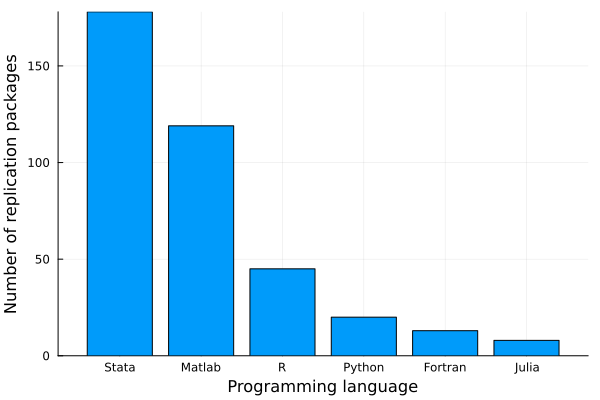
\includegraphics[width=0.45\textwidth]{languages.png}
\caption{Programming language usage in economics replication packages submitted to the Review of Economic Studies. A package can contain code in multiple languages.}
\label{fig:languages}
\end{figure}

Stata and MATLAB are often used together in the same replication package, with Stata focusing on data manipulation and analysis, while MATLAB handles computationally intensive tasks like model simulations. These findings highlight both the current dominance of proprietary scientific computing languages in economics and the large untapped potential for open source tools like Julia. Lowering the barriers to entry through familiar interfaces, as Kezdi.jl aims to do for Stata users, could play an important role in accelerating adoption.

Stata in particular has a dominant position in the data analysis and statistical modeling stages of the research workflow. The vast majority of code in a typical replication package with Stata scripts are devoted to data wrangling and related programming tasks. This is no surprise, given that a typical empirical economics paper assembles and harmonizes data from several disparate sources and the numerous judgment calls that go into this process \cite{huntington2021influence}.

The transition from proprietary languages like Stata or MATLAB to open-source ones like Julia presents several challenges. First, the syntax and mental model is very different. Stata is a data-centric language, where commands operate directly on columns of a dataset, and the details of the type system are hidden from the user. Second, Stata has had decades to build a rich library of statistical and econometric routines that are part of the core language. Third, they have developed coding styles and best practices that are familiar with economists. To name a concrete example, in Stata one can calculate a heteroskedasticity-robust standard error in a regression by simply adding the option \texttt{robust} to the \texttt{regress} command. Achieving the same in Julia requires selecting the appropriate regression function from a package like \texttt{GLM.jl}, exploring the documentation, and, finally, passing the correct arguments.

\texttt{Kezdi.jl} \footnote{\url{https://docs.koren.dev/Kezdi.jl/}} is a data analysis package for economists that aims to ease the transition to Julia by providing a Stata-like user experience. It allows users to manipulate data frames and conduct statistical analysis using Stata-inspired macro commands that are both powerful and easy to read.\footnote{Stata\textsuperscript{\textregistered} is a registered trademark of StataCorp LLC. This package implements command syntax similar to Stata\textsuperscript{\textregistered} but is not affiliated with, endorsed by, or sponsored by StataCorp LLC. Any reference to Stata\textsuperscript{\textregistered} is for informational purposes only and does not imply any relationship with or endorsement by StataCorp LLC.}

\section{Key features of \texttt{Kezdi.jl}}

The overarching design principle of \texttt{Kezdi.jl} is to provide a convenient and familiar interface for economists working with data frames. Here we highlight some key features that help achieve this.

\subsection{Stata-like command syntax}

\begin{figure}[h!]
\begin{lstlisting}[language = Julia, numbers=left, numberstyle=\tiny\color{gray}]
@use "trade.dta"
@generate log_trade = log(trade)
@regress log_trade log_distance, robust
\end{lstlisting}
\caption{Commands in Kezdi.jl follow Stata naming conventions and syntax. All commands start with the \texttt{@} sign. Options are separated from arguments by a comma.}
\label{fig:syntax}
\end{figure}

\texttt{Kezdi.jl} has a good coverage of Stata's data manipulation commands, including \texttt{egen}, \texttt{collapse}, \texttt{reshape} and \texttt{mvencode}. Combined with Julia's superior performance, this allows economists to easily translate their Stata workflows. Some examples of common data wrangling tasks in Kezdi.jl:

\begin{figure}[h!]
\begin{lstlisting}[language = Julia, numbers=left, numberstyle=\tiny\color{gray}]
@generate y = cond(x > 10, 1, 0)
@rename oldname newname
@mvencode y1 y2 y3 @if x < 0, mv(999)
@collapse avg_x = mean(x), by(group)
@reshape long y, i(id) j(year)
\end{lstlisting}
\caption{Some data wrangling commands illustrating the syntax of Kezdi.jl.}
\label{fig:wrangling}
\end{figure}

\subsection{Automatic column selection and vectorization}

Variable names are automatically matched to DataFrame column names in \texttt{Kezdi.jl}. In standard Julia one would need to refer DataFrame columns with \texttt{df[:x]} or \texttt{df.x}. In other helper packages like \texttt{DataFramesMeta.jl} \cite{DataFramesMeta}, one would need to refer to columns with symbols or strings.

Function calls are also automatically vectorized. In the examples above, \texttt{log(trade)} is equivalent to \texttt{log.(trade)} and \texttt{cond(x > 10, 1, 0)} is equivalent to \texttt{cond.(x .> 10, 1, 0)} in base Julia. The \texttt{cond} function returns 1 if the condition is true and 0 otherwise. This is similar to Stata's \texttt{cond()} function. Users can stop vectorization by adding a \texttt{\~} before the function name, like \texttt{\~{}log(trade)}.

Note that not all functions are vectorized. Statistical aggregation functions like \texttt{mean()} and \texttt{sum()} operate on the entire column by default and not elementwise. Any function that takes a \texttt{Vector} as its first argument is not vectorized by default. Users can manually vectorize these functions by adding a dot after the function name.

This way the user has full control over the vectorization of their code. We believe these sensible default behaviors allow for concise and readable code.

\subsection{Use any Julia function}

Because \texttt{Kezdi.jl} supports arbitrary Julia syntax within commands, user-defined and external package functions work seamlessly with DataFrame columns.

\begin{figure}[h!]
\begin{lstlisting}[language = Julia, numbers=left, numberstyle=\tiny\color{gray}]
using Dates
@generate date = Date(year, month, day)

using Statistics
@collapse std_x = std(x), by(group) 
\end{lstlisting}
	
\caption{Any existing or user-defined function can be used in \texttt{Kezdi.jl} code. These are also vectorized automatically.}
\label{fig:vectorization}
\end{figure}

This allows economists to easily extend their data manipulation and modeling capabilities beyond Stata's built-in functions by leveraging Julia's package ecosystem. Users can also write their own functions in Julia and use them in \texttt{Kezdi.jl} commands. 

\subsection{Handling of missing values}
Missing values are a common pain point in data analysis. Julia requires users to handle missing values explicitly, which can be cumbersome, even if it less error-prone. Stata has special rules for the propagation of missing values. For example, \texttt{sum(x)} in Stata returns the sum of non-missing values of \texttt{x}. This is less explicit but more convenient for users.

We follows these rules to handle missing values:
\begin{enumerate}
\item Mathematical operations return \texttt{missing} if any of their arguments are missing. This is also true for functions that do not support missing values. For example, \texttt{log(missing)} returns \texttt{missing}.
\item Aggregation functions skip missing values by default. For example, \texttt{sum(x)} returns the sum of non-missing values of \texttt{x}.
\item In logical expressions, \texttt{missing} is treated as \texttt{false}. This is unlike Stata, where \texttt{missing} is treated as \texttt{true}. This is a conscious decision to avoid common pitfalls with missing values.
\end{enumerate}

\begin{figure}[h!]
\begin{lstlisting}[language = Julia, numbers=left, numberstyle=\tiny\color{gray}]
using Kezdi
df = DataFrame(x=[1, 2, missing], y=[missing, 3, 4])
@collapse sum_x = sum(x)
# returns 3

@generate z = x + y
# returns [missing, 5, missing]
\end{lstlisting}
	
\caption{Missing values are handled in a logical way.}
\label{fig:missing}
\end{figure}

\subsection{Syntactic sugar for operating on a subset of rows}

One of the most convenient features of Stata is the ability to restrict any command to a subset of rows using logical expressions with the \texttt{if} qualifier. \texttt{Kezdi.jl} implements the same with the \texttt{@if} macro.\footnote{Even though \texttt{@if} looks like a macro, it is not implemented as one, because \texttt{if} is a reserved word in Julia. The macro call is processed during parsing the \texttt{Kezdi.jl} command.} 

\begin{figure}[h!]
\begin{lstlisting}[language = Julia, numbers=left, numberstyle=\tiny\color{gray}]
@replace trade = 0 @if ismissing(trade)
@regress log_trade log_distance @if trade > 0
@keep @if !ismissing(trade) 
@collapse mean_x = mean(x) @if group == "treatment"		
\end{lstlisting}
\caption{The @if macro can be used to limit the scope of any command.}
\label{fig:ifmacro}
\end{figure}

\subsection{Integration with Julia's package ecosystem}

\texttt{Kezdi.jl} builds on the \texttt{DataFrames.jl} ecosystem \cite{DataFrame.jl2023} to provide its data manipulation features. It also integrates tightly with other packages:

\begin{enumerate}
	\item \texttt{FreqTables.jl} \cite{FreqTables.jl2023} for frequency tables via \texttt{@tabulate}
	\item \texttt{FixedEffectModels.jl} \cite{FixedEffectModels.jl2023} for estimating regressions with \texttt{@regress}
	\item \texttt{Chain.jl} \cite{Chain} for piping a sequence of commands with \texttt{@with}
	\item \texttt{ReadStatTables.jl} \cite{ReadStatTables} for importing Stata \texttt{.dta} files
\end{enumerate}

\section{Comparison with related packages}
\texttt{Kezdi.jl} is not the first attempt to provide a simplified data analysis workflow in Julia. \texttt{DataFramesMeta.jl} \cite{DataFramesMeta} extends the DataFrame interface with easy-to-use macros. On the R side, dplyr \cite{dplyr2023} has been a hugely successful abstraction. \texttt{TidierData.jl} \cite{tidier2022} ports many ideas from dplyr to Julia and served as a primary inspiration for many of our design choices. 

texttt{Douglass.jl} is a related package that also aims to provide a Stata-like user experience in Julia \cite{Douglass.jl2023}. The two packages share similar goals, but \texttt{Kezdi.jl} has a more extensive feature set and is more actively developed.

\section{Conclusion}

We introduced \texttt{Kezdi.jl}, a data analysis package for economists that provides a Stata-like interface to Julia's data manipulation and statistics ecosystem. \texttt{Kezdi.jl} aims to shorten the learning curve for economists transitioning from Stata, while also unlocking the power and expressiveness of Julia.

With \texttt{Kezdi.jl}, economists can manipulate data frames, calculate summary statistics, and estimate regressions using familiar keystrokes and mental models. At the same time, the package opens the door to Julia's rich ecosystem of packages for optimization, machine learning, visualization, and high-performance computing.

Our hope is that \texttt{Kezdi.jl} will accelerate adoption of Julia in economics and other social sciences, and ultimately lead to better, more reproducible research. We invite researchers and developers to try out the package and share their feedback on how we can expand its capabilities to better meet their scientific computing needs.

\section*{Acknowledgments}

The package is named in memory of Gábor Kézdi\footnote{\url{https://kezdigabor.life}}, a prominent applied microeconomist and advocate of democratizing data analysis tools \cite{gabors-data}. We are grateful to the Julia community for their support and feedback, and to the Review of Economic Studies for hosting the replication packages that inspired this work.

% **************GENERATED FILE, DO NOT EDIT**************

\bibliographystyle{juliacon}
\bibliography{ref.bib}

\end{document}
